\documentclass[vmargin=1cm]{article}
\usepackage[siunitx, european, american currents]{circuitikz}
\usepackage{subcaption}

% Style global pour atténuer le reste du circuit
\tikzset{dimmed/.style={opacity=0.2, gray}}
\tikzset{highlight/.style={ultra thick, draw=red}}

\begin{document}

\begin{figure}[h]
    \centering
    % --- GRAPHE 1 : RÉFÉRENCE ---
    \begin{subfigure}{0.45\textwidth}
        \centering
        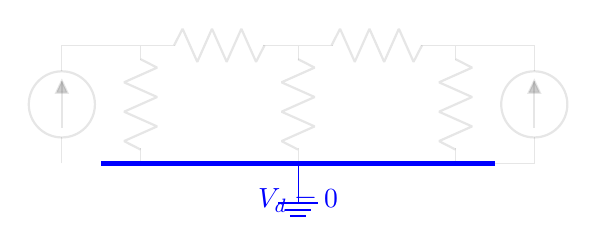
\begin{tikzpicture}[american, scale=0.5]
            \coordinate (d) at (0,0); \coordinate (a) at (-4,3); \coordinate (b) at (0,3); \coordinate (c) at (4,3);
            \draw[dimmed] (-6,0) to[I] (-6,3) -- (a) to[R] (a |- d);
            \draw[dimmed] (a) to[R] (b) to[R] (d) (b) to[R] (c) to[R] (c |- d) -- (6,0) to[I] (6,3) -- (c);
            % Highlight
            \draw[blue, ultra thick] (-5,0) -- (5,0);
            \node[ground, color=blue, scale=1.2] at (d) {};
            \node[below=2mm, blue] at (d) {$V_d = 0$};
        \end{tikzpicture}
        \caption{Mise à la terre (Référence)}
    \end{subfigure}
    \hfill
    % --- GRAPHE 2 : PASSIFIÉ ---
    \begin{subfigure}{0.45\textwidth}
        \centering
        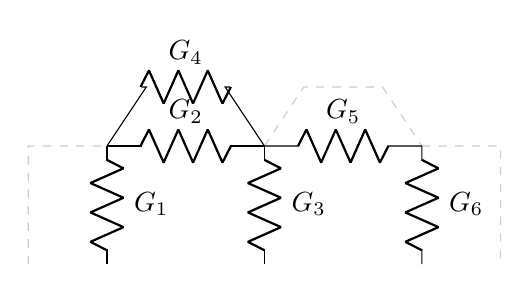
\begin{tikzpicture}[american, scale=0.5]
            \coordinate (d) at (0,0); \coordinate (a) at (-4,3); \coordinate (b) at (0,3); \coordinate (c) at (4,3);
            % On dessine tout SAUF les sources (circuits ouverts)
            \draw (a) to[R, l=$G_1$] (a |- d) (a) to[R, l=$G_2$] (b) (b) to[R, l=$G_3$] (d);
            \draw (b) to[R, l=$G_5$] (c) (c) to[R, l=$G_6$] (c |- d) (a) -- (-3,4.5) to[R, l=$G_4$] (-1,4.5) -- (b);
            \draw[dashed, opacity=0.2] (-6,0) -- (-6,3) -- (a) (b) -- (1,4.5) -- (3,4.5) -- (c) (c) -- (6,3) -- (6,0);
        \end{tikzpicture}
        \caption{Graphe Passifié (Sources éteintes)}
    \end{subfigure}

    \vspace{1cm}

    % --- GRAPHE 3 : SOURCES ---
    \begin{subfigure}{0.45\textwidth}
        \centering
        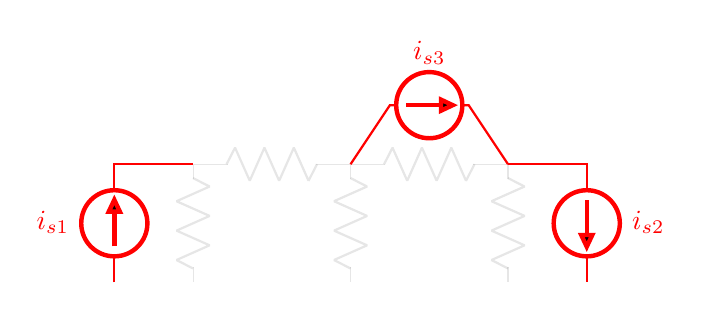
\begin{tikzpicture}[american, scale=0.5]
            \coordinate (d) at (0,0); \coordinate (a) at (-4,3); \coordinate (b) at (0,3); \coordinate (c) at (4,3);
            \draw[dimmed] (a) to[R] (a |- d) (a) to[R] (b) to[R] (d) (b) to[R] (c) (c) to[R] (c |- d);
            % Highlight sources
            \draw[red, thick] (-6,0) to[I, l=$i_{s1}$] (-6,3) -- (a);
            \draw[red, thick] (b) -- (1,4.5) to[I, l=$i_{s3}$] (3,4.5) -- (c);
            \draw[red, thick] (c) -- (6,3) to[I, l=$i_{s2}$] (6,0);
        \end{tikzpicture}
        \caption{Sources de courants}
    \end{subfigure}
    \hfill
    % --- GRAPHE 4 : POTENTIELS ---
    \begin{subfigure}{0.45\textwidth}
        \centering
        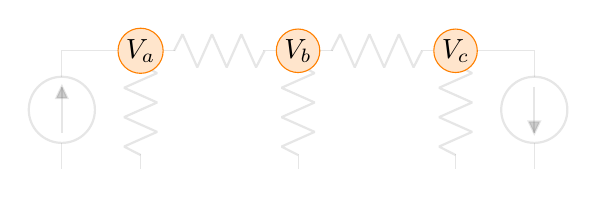
\begin{tikzpicture}[american, scale=0.5]
            \coordinate (d) at (0,0); \coordinate (a) at (-4,3); \coordinate (b) at (0,3); \coordinate (c) at (4,3);
            \draw[dimmed] (-6,0) to[I] (-6,3) -- (a) to[R] (a |- d) (a) to[R] (b) to[R] (d) (b) to[R] (c) (c) to[R] (c |- d) (c) -- (6,3) to[I] (6,0);
            % Highlight Noeuds
            \node[circle, fill=orange!20, draw=orange, inner sep=1pt] at (a) {$V_a$};
            \node[circle, fill=orange!20, draw=orange, inner sep=1pt] at (b) {$V_b$};
            \node[circle, fill=orange!20, draw=orange, inner sep=1pt] at (c) {$V_c$};
        \end{tikzpicture}
        \caption{Potentiels de nœuds}
    \end{subfigure}
\end{figure}

\end{document}